\documentclass[../thesis.tex]{subfiles}
\begin{document}
\chapter{Transient and Steady-State Dynamics}

This section is an extension of my previous work entitled ``\textit{Unified analysis of transient and steady-state electrophosphorescence using exciton and polaron dynamics modeling}''.\cite{Hershey2016}

\section{Motivation}

As discussed in Chapter \ref{sec:oleds}, modern OLEDs are typically based around Phosphorescent emitters in order to realize 100\% internal efficiencies.\cite{Baldo2000,Baldo1998a,Tsutsui1999,OBrien1999a}
However, these phosphorescent emitters, while allowing emission out of the triplet excitonic state, also suffer from the drawback of a longer exciton lifetime, typically on the order of 10$^{-6}$-10$^{-3}$ s.\cite{Baldo1998a,Holmes2003}
An increased lifetime leads to a larger steady-state triplet exciton density compared to a fluorescent device operating at the same luminance.  
This becomes problematic at the high current densities associated with high brightness due to well documented quenching events.\cite{Reineke2007,Reineke2007a,Reineke2009,Mezyk2005,Kalinowski2002,Song2010,Erickson2014}
These quenching events lead to a reduced quantum efficiency at high-current, and termed the ``Efficiency roll-off''.  

\begin{wrapfigure}{R}{0.5\textwidth}
\centering
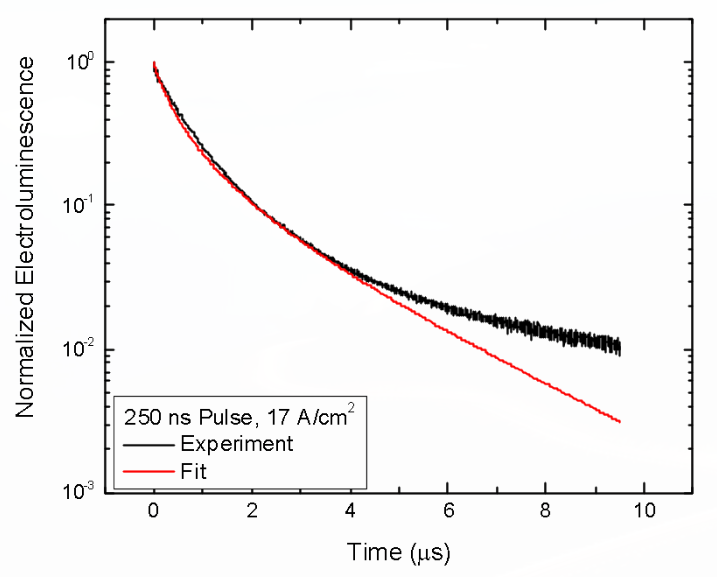
\includegraphics[width=0.48\textwidth]{unified/bad_fit}
\caption{Fitting the transient electroluminescence decay without polaron dynamics.}
\label{fig:bad_fit}
\end{wrapfigure}

Efficiency roll-off is well attributed to quenching and is ubiquitous to phosphorescent OLED behavior.\cite{Reineke2007,Erickson2014,Murawski2013,Giebink2008c}
While previous works have attributed the roll-off to quenching, they have failed to provide a complete picture of the exciton and charge dynamics within the device.
All of these works have utilized a differential equations model for the exciton dynamics, solved in the steady state.
This becomes apparent when investigating the transient electroluminescnce (EL), where a transient voltage pulse, on the order of 500 ns is applied to the device and the resulting luminance is recorded as a function of time.  
Figure \ref{fig:bad_fit} is an attempt to fit the transient luminance decay using the model presented by Reineke \textit{et al.} which well fits the efficiency roll-off.  Indeed, this is a well known problem with existing models, and previous attempts to model the transient EL have utilized an empirical biexponential function to quantifiy the decay.\cite{Erickson2014,Giebink2008c,Baldo2000a,Zhang2012}
In addition to failing to replicate the luminance decay, no known previous efforts have been made in trying to replicate the experimental transient EL luminance rise.

\begin{wrapfigure}{R}{0.5\textwidth}
\centering
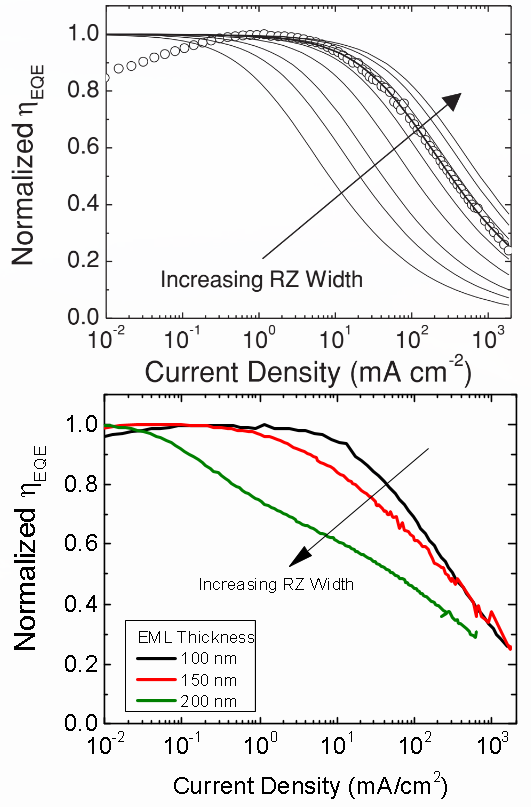
\includegraphics[width=0.48\textwidth]{unified/rz_dependence}
\caption{(a) Efficiency roll-off predicted by Erickson \textit{et al.} 2014 as a function of recombination zone width. (b) Observed efficiency roll-off for gradient EML devices.}
\label{fig:rz_dependence}
\end{wrapfigure}

In addition to the problems with the transient electroluminescence, the interpretation of the existing model without a full dynamics picture can lead to false predictions.  
Figure \ref{fig:rz_dependence}a shows what a quenching model predicts for the roll-off as a function of increasing recombination zone width.  
However, even in the most idealized case of a gradient emissive layer device, where no additional interfaces come into play, the predictive model fails to replicate the behavior, as shown in Figure \ref{fig:rz_dependence}b.
While this device is of little interest for further investigation due to the extreme thickness, the point stands that this model has glaring assumptions for it's applications.

Both the transient EL and the recombination zone dependence issues arise due to an incomplete picture of the device physics, more specifically in the area of polaron dynamics.  
This work sought to address these issues by including polaron dynamics.  
Since the steady-state solution of existing models is able to accurately replicate steady-state performance, the transient EL is utilized as well as the steady-state solution to ensure that the underlying physics are accurately captured.
A valid solution should be able to accurately fit both regimes using the same model parameter values.
In order to leverage previous work, the archetypical green-emitter tris[2-phenylpyridinato-c$_2$,N]Iridium(III) (Ir(ppy)$_3$) is used for the extensively characterized photophysics.\cite{Baldo2000,Baldo2000a,Tsuboi2006,Adachi2001a,Kawamura2006,Kawamura2005c}

%---------------------------------------------------------------------------------------------
\section{Theory}
\subsection{Exciton Dynamics}
The dominannt processes that influence the exciton population, first formalized by Reineke \textit{et al.}\cite{Reineke2007}, have been identified as natural exciton decay, via radiative and non-radiative processes, triplet-triplet annihilation, triplet-polaron quenching, and exciton generation.\cite{Erickson2014,Song2010}
In triplet-triplet annihilation, two triplets are able to interact, and one exciton transfers its energy to the other, resulting in one molecule relaxing to the ground state and the other forming a hot excited state.
This hot state releases this additional energy to heat and typically relaxes back to the $T_1$ state.  
Triplet-polaron quenching is the interaction of a polaron with a nearby triplet exciton.
Here, one of the charges of the exciton non-radiatively recombines with the polaron of the opposite charge, leaving a remaining loose charge.
Excitons are also subject to field dissociation, but this mechanism is ignored in this work.
Field dissociation is typically observed for fields larger than $2.5 \times 10^6$ V/cm.  
This is near the maximum field used for this study, and would be important to consider for higher voltage characterization.

In agreement with previous models, singlet-triplet exciton intersystem crossing and host-guest exciton energy transfer are assumed to be fast compared to exciton decay.\cite{Reineke2007,Baldo2000a,Turro1991a}
Since these mechanisms are much faster, they will not be rate-limiting processes and can thus be omitted from the differential equations model without sacrificing accuracy.
Within an operational device, electron and hole populations are indistinguishable.
Therefore, the electron ($n_e$) and hole ($n_h$) densities are treated as a single geralized polaron population, $n_{pol}=n_e+n_h$.
For simplicity, the model developed here treats the exciton and polaron populations as spatially uniform and confined to the exciton recombination zone.  An spatial inhomogeneity in exciton and polaron density as well as their overlap is absorbed into the bimolecular rate constants.
It is important to note that due to this assumption, rate constants are a property of the device stack, and not just a material property.
With these assumptions, the dynamic processes determining exciton density ($n_{ex}$) can be summarized in the following one-dimensional rate equation:

\begin{equation}
%\frac{dn_{ex}}{dt} = - \frac{n_{ex}}{\tau}-\frac{1}{2}k_{TT}n_{ex}^2-k_{TP}n_{pol}n_{ex}+G_{ex}
\frac{dn_{ex}}{dt} = - \frac{n_{ex}}{\tau}-\frac{1}{2}\ktt n_{ex}^2-\ktp n_{pol}n_{ex}+G_{ex}
\label{eqn:exciton_rate}
\end{equation}

where $\tau$ is the natural exciton lifetime, determined by the radiative ($k_r$) and non-radiative ($k_{nr}$) decay rates by $\tau=1/(k_r+k_{nr})$, \ktt is the rate constant for triplet-triplet annihilation, \ktp is the rate constant for triplet-polaron quenching, and $G_{ex}$ is the exciton generation rate.  
As this is a one-dimensional model, $G_{ex}$ is a spatially uniform generation rate, a simplifying assumption.
Many studies have modeled the exciton recombination zone profile, relying on material energy levels, as well as mobilities.\cite{Rihani2006,Hassine2001,Hassine2002,Ruhstaller2003,Ruhstaller2001}
While these models are more accurate and explicit, in the way that they capture the physics, they also increase the dimensionality of our model, as well as increasing the parameterization; requiring seperate electron and hole rate equations, mobilities and energy levels for every material.
Even with this increased accuracy of the physical processes, identifying if the predicted exciton recombination zone is accurate requires significant additional measurements.
Since the goal of this work is to provide a functional model to accurately predict the transient and steady-state device behavior, spatially uniform dynamics are assumed.
Here, exciton formation is treated using a Langevin recombination formalism based on the polaron density.\cite{Ruhstaller2003,Pinner1999,Blom1996}

\begin{equation}
G_{ex}=\frac{\kf}{4}n_{pol}^2
\label{eqn:exciton_formation}
\end{equation}

where \kf is the rate constant for exciton formation.  The factor of four accounts for the diversity of the polaron population and assumes that electrons and holes are in equal proportion.  
The accuracy of this prefactor is reduced for imbalanced charge, and is investigated in Section \ref{sec:charge_imbalance}.
For $n_e$:$n_h$ ratios 2:1 or better, less than 20\% error is found in this term.  

\section{Polaron Dynamics}

Previous models for efficiency roll-off have ignored polaron dynamics and assumed that all polarons readily form excitons.  The steady-state polaron density is then modeled using a space charge limited model.\cite{Pope1999}
To attribute physics to this process, a simple picture of polaron dynamics is assumed, consisting of charge injection and transport, exciton formation, and polaron loss.  
In order to preserve our one-dimensionality, polarons must be uniformly distributed.  
Without competing losses in the tranport layers, all injected polarons must eventually reach the emissive layer.  
We further assume that polarons easily enter that emissive layer and that the majority of polaron build up occurs within the emissive layer, rather than the transport layers.
Therefore, the charges injected from the current density, $J$, are uniformly generated in the emissive layer by $G_{pol}=2J/ew$.  Here, $e$ is the electron charge, and the factor of two arises from an assumption of equal charge injection.  In a well balanced device, the measured current forms holes on one side of the device and electrons on the other, and are both injected into the device.  
This is discussed extensively in Section \ref{sec:carrier_injection}
Polaron losses to exciton formation mirror the exciton formation rate presented in Equation \ref{eqn:exciton_formation}, though at twice the rate due to two polarons forming one exciton.

The introduction of polaron loss from the emissive layer through the device without forming excitons is essential to address the limitations of previous models.  
Without this term, peak internal quantum efficiency of all devices is assumed to be 100\% and and the roll-up of efficiency at low current can not be explained.  
In order to capture polaron loss, a first order approximation is made for loss in that only the majority charge carrier can be lost and leaks through the device with a characteristic time, $\tau_l$.
With these mechanisms, the full polaron dynamics can be expressed as:




\begin{equation}
\frac{dn_{pol}}{dt}=\frac{-\kf}{2}n_{pol}^2-\frac{n_{pol}}{\tau_l}+G_{pol}.
\label{eqn:polaron_rate}
\end{equation}

\section{Exciton Quenching in Photoluminescence}

\begin{equation}
V=\left[ \frac{J}{e\mu N_C}d^{2l+}\left( \frac{eN_0k_BT_t}{\epsilon} \right)^l \right]^{\frac{1}{l+1}}=CJ^{\frac{1}{l+1}}
\label{eqn:ktpVoltage}
\end{equation}

\begin{equation}
n_{pol}=eN_c\left(\frac{\epsilon V}{ed^2N_0kT_t}\right)^l
\label{eqn:kptDensity}
\end{equation}

\begin{equation}
\frac{L(n_{pol}}{L_0}=\frac{1}{1+\tau \ktp n_{pol}}
\label{eqn:ktpFit}
\end{equation}




\begin{wrapfigure}{R}{0.5\textwidth}
\centering
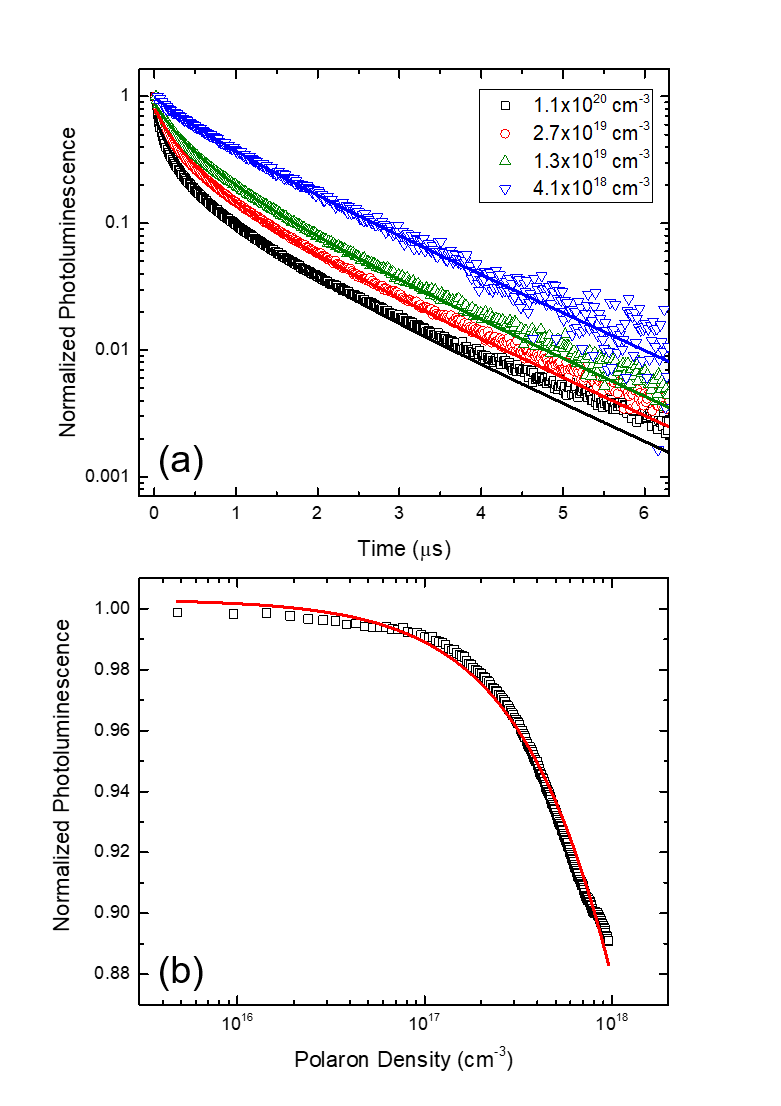
\includegraphics[width=0.48\textwidth]{unified/PL_fitting}
\caption{(a) Transient photoluminescence (PL) decays for several initial exciton densities with fits shown as solid lines using Eqn. \ref{eqn:exciton_formation}.  Fit parameters are discussed in SECTION.  Exciton densities are calculated using measured incident power and beam size in combination iwht Beer's Law.  (b) Steady-state PL quenching as a function of polaron density and the resulting fit from Eqn. \ref{eqn:ktpFit} shown as the solid line.}
\label{fig:PL_fitting}
\end{wrapfigure}
\subsection{Transient Electroluminescence}
\subsection{Efficiency Analysis}

\begin{equation}
%\eta_{EQE}=\eta_{OC}\eta_{PL}\chi\eta_{EF}
\eqe=\oc \pl \chi \ef
\label{eqn:eqeSimple}
\end{equation}

\begin{equation}
%\eta_{EQE}=\frac{\eta_{OC}\eta_{ex}k_r}{G_{pol}/2}
\eqe=\frac{\oc n_{ex}k_r}{G_{pol}/2}
\label{eqn:eqeReform}
\end{equation}

\begin{equation}
\ef=\frac{\frac{1}{2}\kf n_{pol}}{G_{pol}}=\frac{\frac{1}{2}\kf n_{pol}}{\frac{1}{2}\kf n_{pol}+\frac{1}{\tau_l}}
\label{eqn:excitonFormation}
\end{equation}

\section{Experimental Details}
\section{Application to Devices}
\subsection{Overview of Approach}
\subsection{Initializing Parameters with Quenching Only Steady-State Model}
\begin{wrapfigure}{R}{0.5\textwidth}
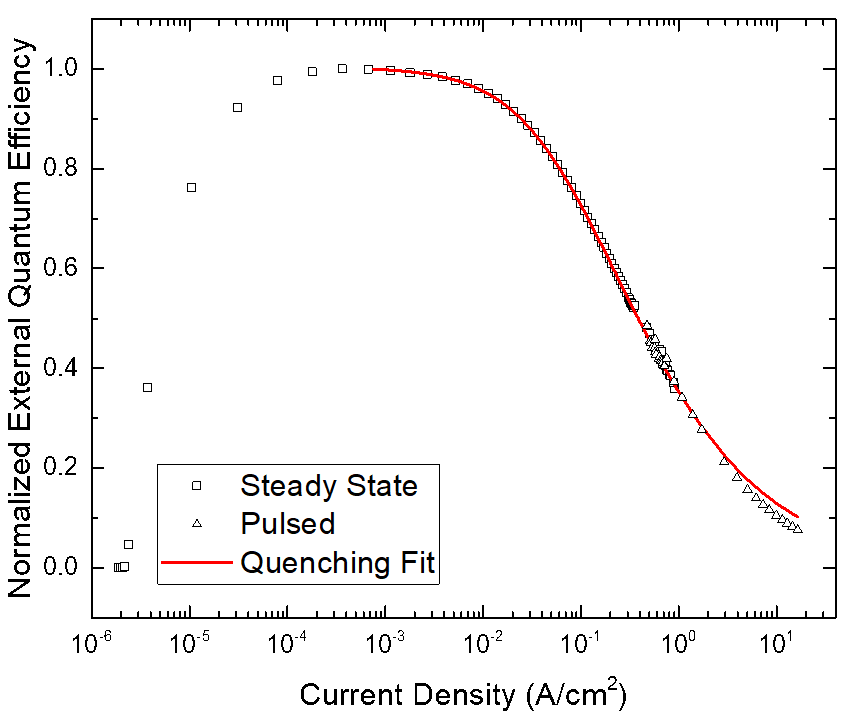
\includegraphics[width=0.48\textwidth]{unified/rollOffFit}
\caption{Normalized experimental \eqe as a function of current density.  Solid line is a fit to the data using Eqn. \ref{eqn:exciton_rate} and \ref{eqn:polaron_rate} in the absence of polaron loss.  Pulsed eqe measurements are conducted using low duty cycle pulses to steady-state luminance to reduce Joule heating in device.}
\label{fig:rollOffFit}
\end{wrapfigure}
\subsection{Transient Modeling}
\begin{wrapfigure}{R}{0.5\textwidth}
\centering
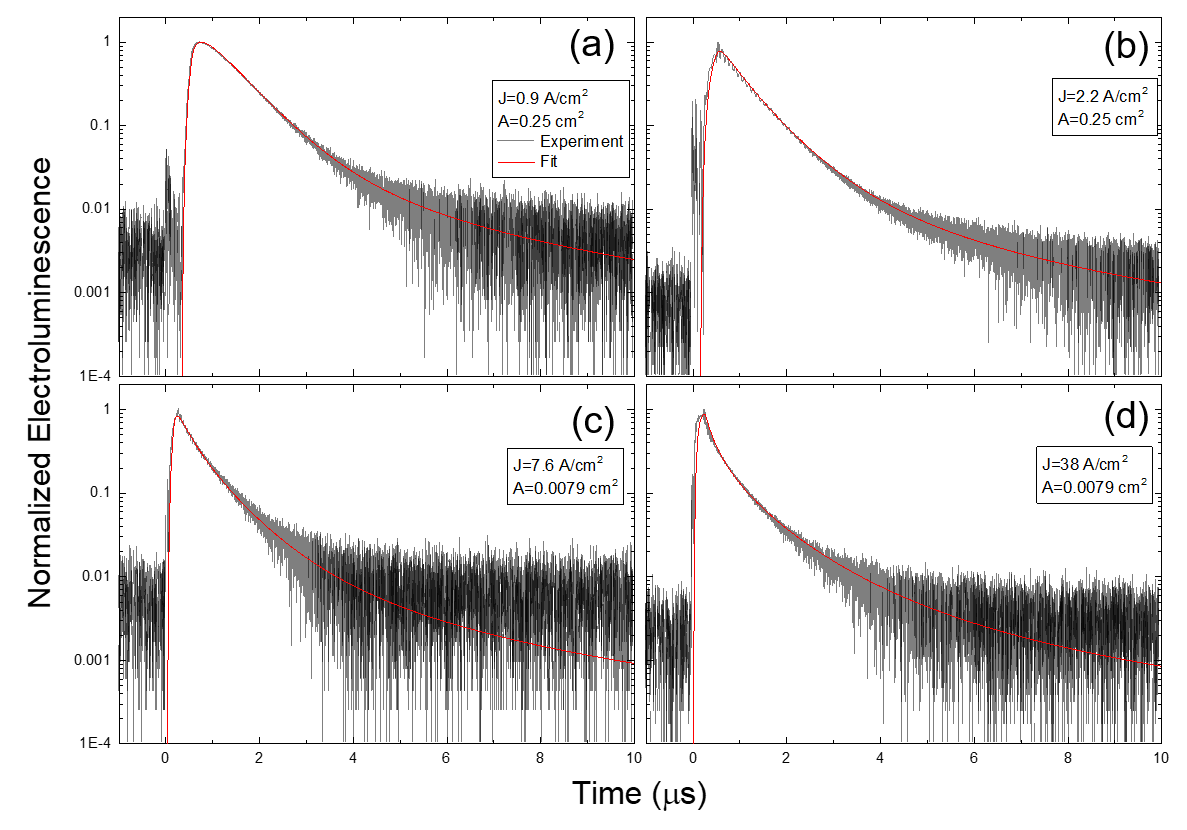
\includegraphics[width=0.48\textwidth]{unified/transientFits}
\caption{Transient electroluminescence (EL) for four different current densities (J) and device areas (A). (a) 0.25 $cm^2$ device at a current density during the pulse of J = 0.9 $A/cm^2$ (b) 0.25 cm2
device at J = 2.2 $A/cm^2$ (c) 0.0079 $cm^2$ device at J = 7.6 $A/cm^2$ (d) 0.0079 $cm^2$ device at J = 38 $A/cm^2$}
\label{fig:transientFits}
\end{wrapfigure}

\begin{table}[h]
\centering
\begin{tabular}{c|c|c}
& Transient EL & Efficiency Roll-off \\
\hline
$\tau$ (s) & $6.9\pm 0.1 \times 10^{-7}$ & $6.1 \times 10^{-7}$ \\
\ktt (cm$^3$/s) & $7.1\times 10^{-12}$ &$7.1\times 10^{-12}$ \\
\ktp (cm$^3$/s) & $3.3\times 10^{-13}$ &$3.3\times 10^{-13}$ \\
\kf (cm$^3$/s) & $7.7\pm3.5\times 10^{-12}$ &$1.6\times 10^{-11}$ \\
\end{tabular}
\caption{Fit parameters extracted from transient and steady-state electroluminescence.  Transient EL fit parameters averaged over all measured current densities.  \eqe roll-off parameters averaged over several measured devices.  Triplet-triplet annihilation and triplet-polaron quenching rates are fixed to those obtained from fitting the normalized efficiency roll-off.}
\label{tab:fit_parameters}
\end{table}
% 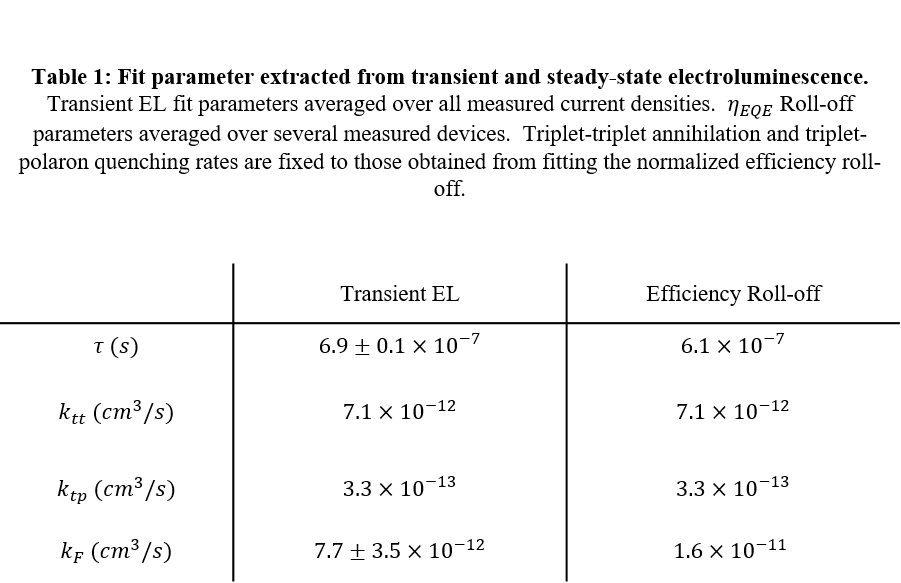
\includegraphics[width=0.48\textwidth]{unified/valueTable}
\subsection{Term Efficiency During Transient}


\begin{wrapfigure}{R}{0.5\textwidth}
\centering
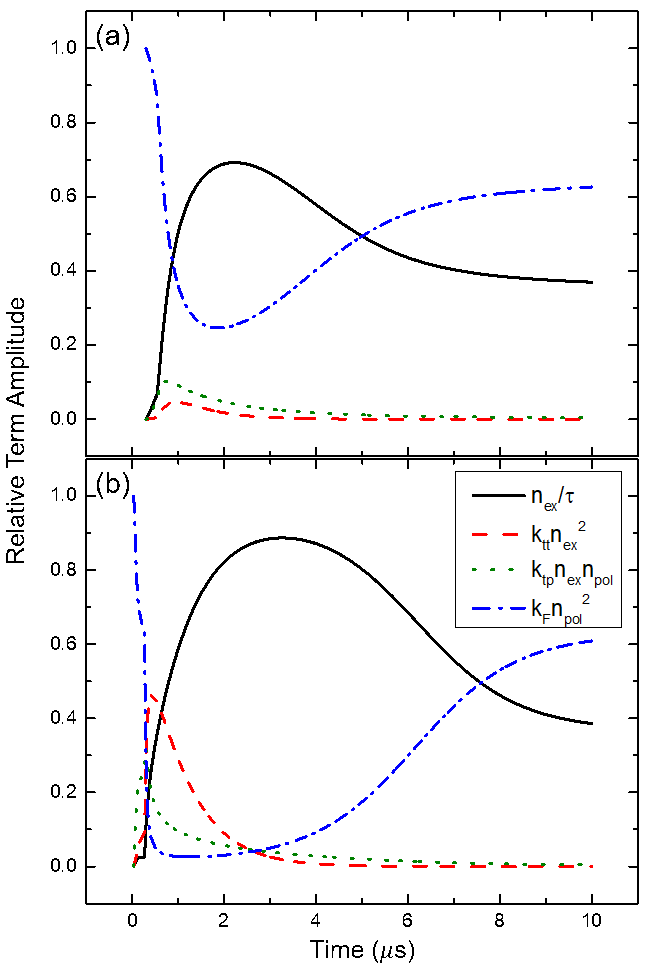
\includegraphics[width=0.48\textwidth]{unified/termEfficiency}
\caption{Term efficiency for each dynamical process influencing the exciton population for (a) 0.25 $cm^2$ device operated at 0.9 $A/cm^2$ for 500 ns and (b) 0.785 $mm^2$ device operated at a current density of 38 $A/cm^2$ for 250 ns. Relative term amplitude is calculated as the magnitude of each term in Eqn. \ref{eqn:exciton_rate} divided by the sum of absolute values of each term.}
\label{fig:termEfficiency}
\end{wrapfigure}
\subsection{Extracting Exciton Formation Efficiency}
\begin{wrapfigure}{R}{0.5\textwidth}
\centering
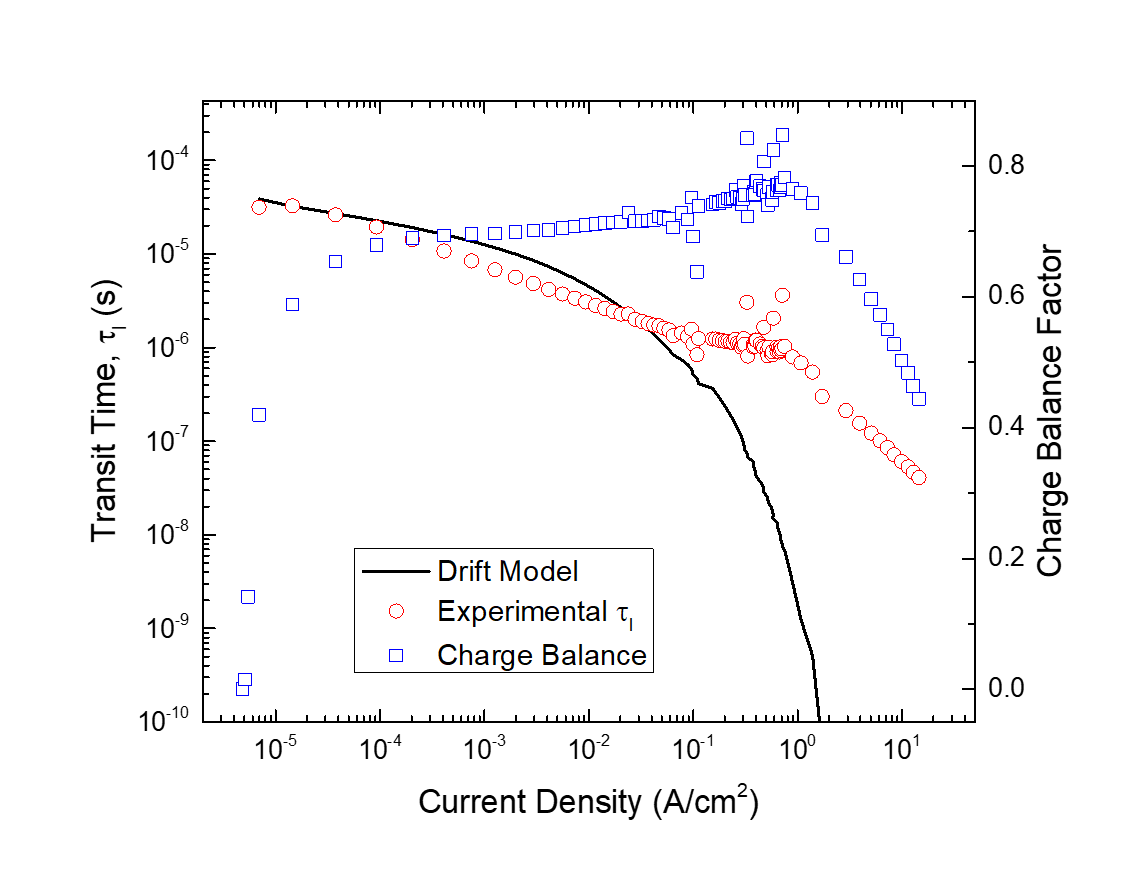
\includegraphics[width=0.48\textwidth]{unified/chargeBalance}
\caption{Transit time extracted from \eqe measurements are shown as the red circles. Predictions using the drift model are calculated using Eqn. \ref{eqn:drift}. The drift model assumes a uniform electric field. Good agreement between the experimental transit time and the drift model is found for a field distributed over 20 nm. The charge balance factor is shown as a function of current density in blue squares.}
\label{fig:chargeBalance}
\end{wrapfigure}
\subsection{Drift Model}

\begin{equation}
\tau_l=\frac{w}{E\mu(E)}
\label{eqn:drift}
\end{equation}


\section{Understanding Assumptions of Polaron Model}
\subsection{Carrier Injection} \label{sec:carrier_injection}

\begin{equation}
\frac{dn_h}{dt}=-\kf n_en_h-\frac{n_h}{\tau_{lh}}+\frac{J_h}{ew}
\label{eqn:hole_rate}
\end{equation}

\begin{equation}
\frac{dn_e}{dt}=-\kf n_en_h-\frac{n_e}{\tau_{le}}+\frac{J_e}{ew}
\label{eqn:electron_rate}
\end{equation}

\begin{equation}
J_1\rightarrow J_h = J_2 \rightarrow J_e
\label{eqn:current_no_leakage}
\end{equation}

\begin{equation}
\frac{J_e}{ew}+\frac{J_h}{ew}=\frac{J_1+J_2}{ew}=\frac{2J}{ew}
\label{eqn:injected_polarons_no_leakage}
\end{equation}

\begin{equation}
J_1=J_h
\label{eqn:current_holes_leakage}
\end{equation}

\begin{equation}
J_2=J_e+J_l
\label{eqn:current_electrons_leakage}
\end{equation}

\begin{equation}
J=J_h=J_e+J_l
\label{eqn:current_continuity_leakage}
\end{equation}

\begin{equation}
G_{pol}-\frac{J_l}{ew}=\frac{2J-J_l}{ew}
\label{polaron_generation}
\end{equation}

\subsection{Charge Imbalance} \label{sec:charge_imbalance}

\begin{equation}
\alpha=\frac{n_h}{n_e+n_h}
\label{eqn:charge_ratio}
\end{equation}

\begin{equation}
\left[\frac{dn_{pol}}{dt}\right]_{formation}=-2\kf n_{pol}^2\alpha(1-\alpha)
\label{eqn:exciton_formation_charge_ratio}
\end{equation}



\begin{wrapfigure}{R}{0.5\textwidth}
\centering
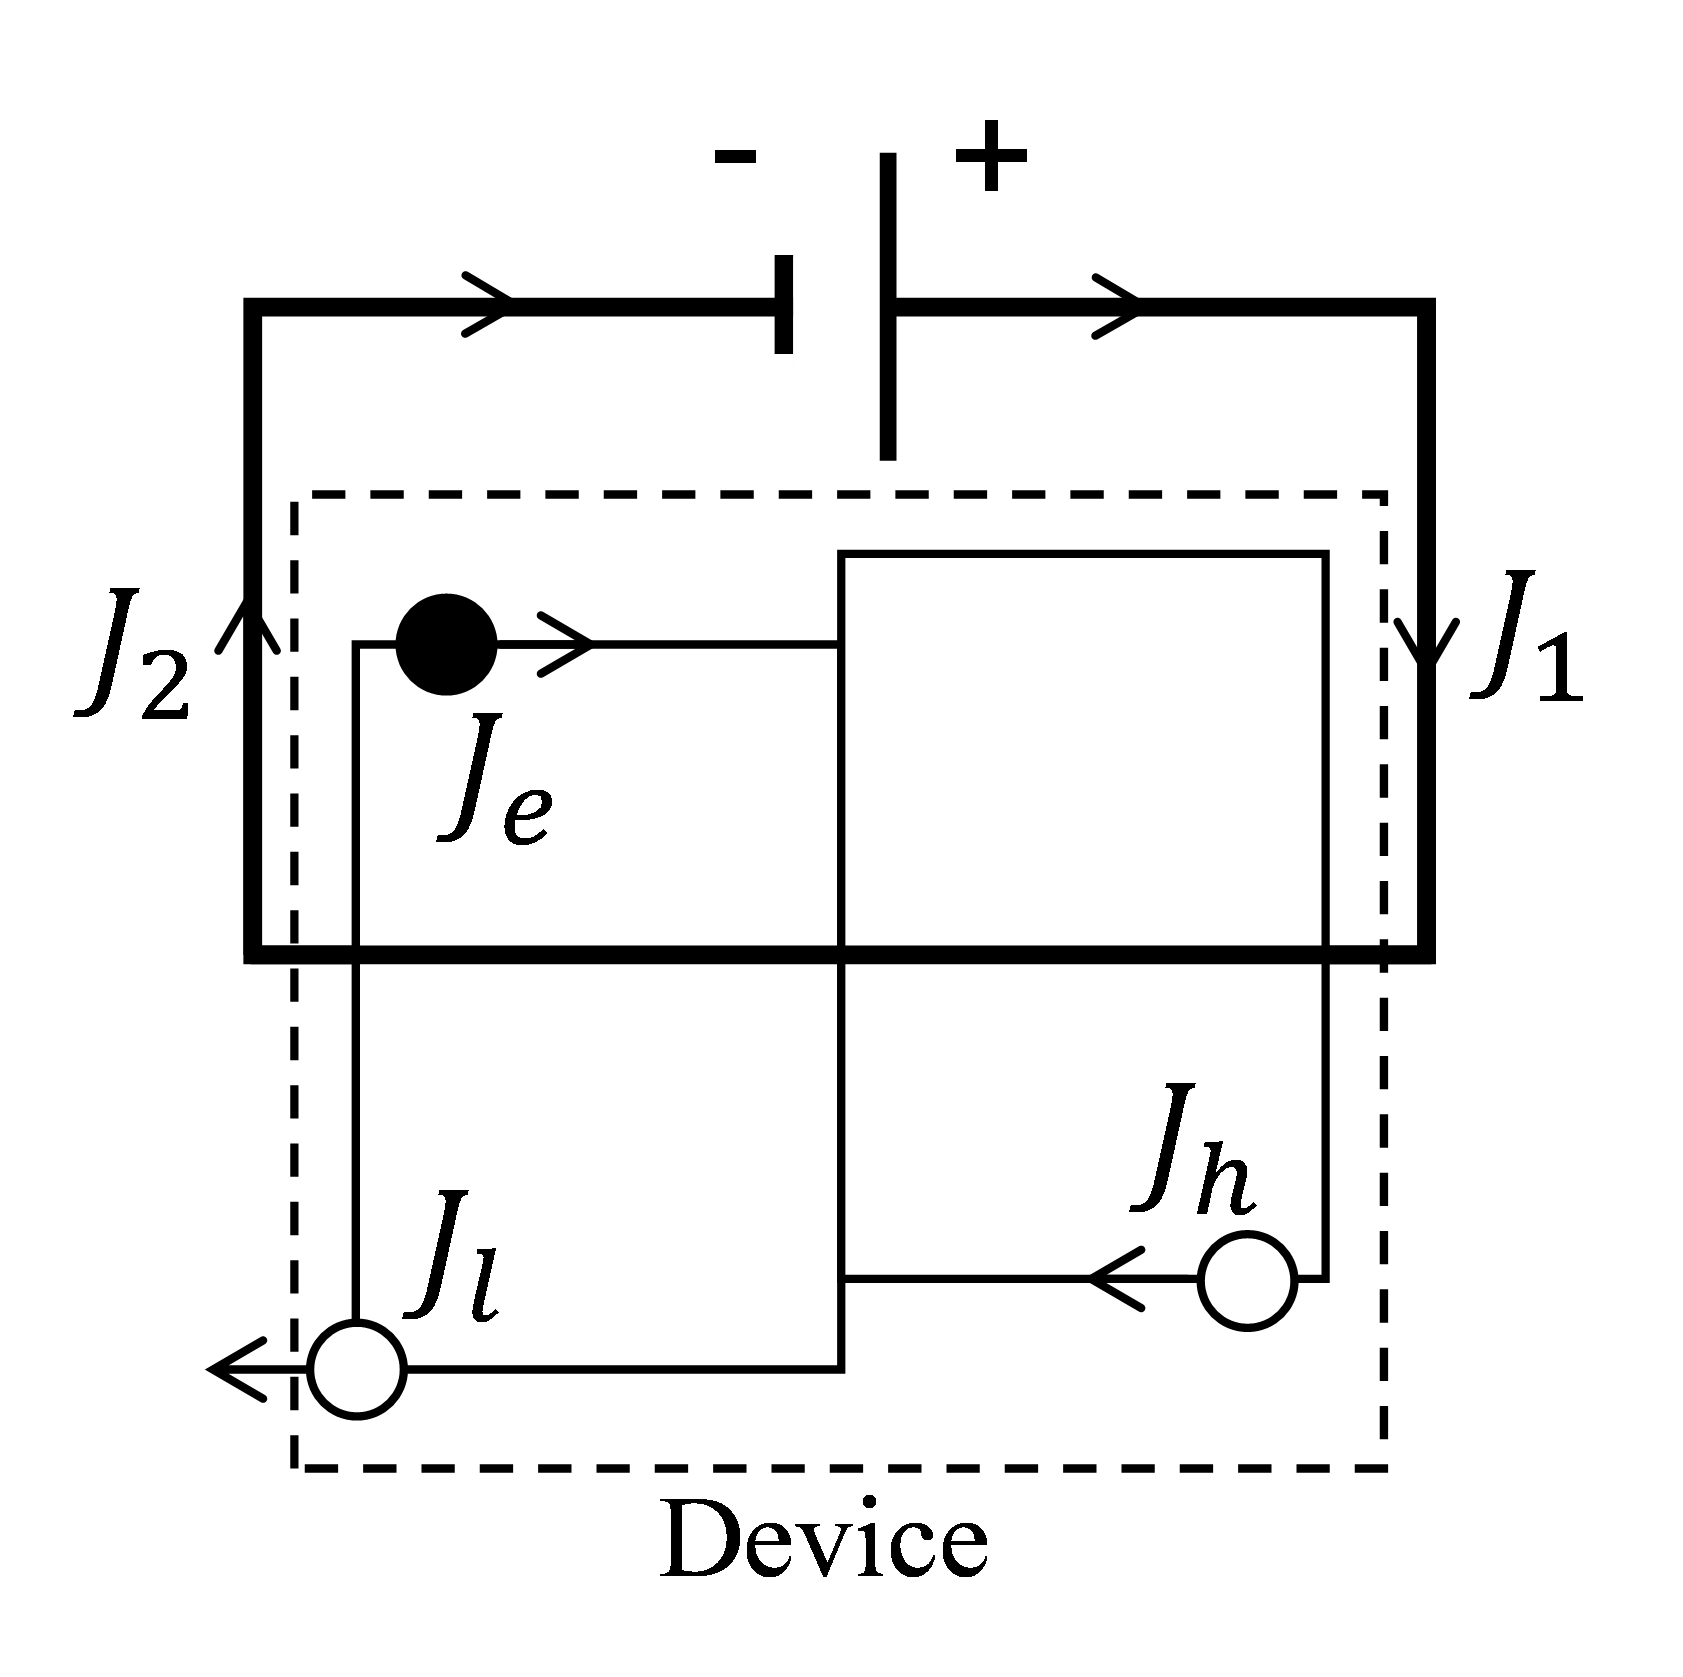
\includegraphics[scale=.1]{unified/currentDiagram}
\caption{Current density formalism within the circuit. and are the currents measured on either side of the device. and are the electron and hole currents within the device and is the unbalanced current, assumed to be only holes, that leaks out of the opposing contact.}
\label{fig:currentDiagram}
\end{wrapfigure}

\begin{wrapfigure}{R}{0.5\textwidth}
\centering
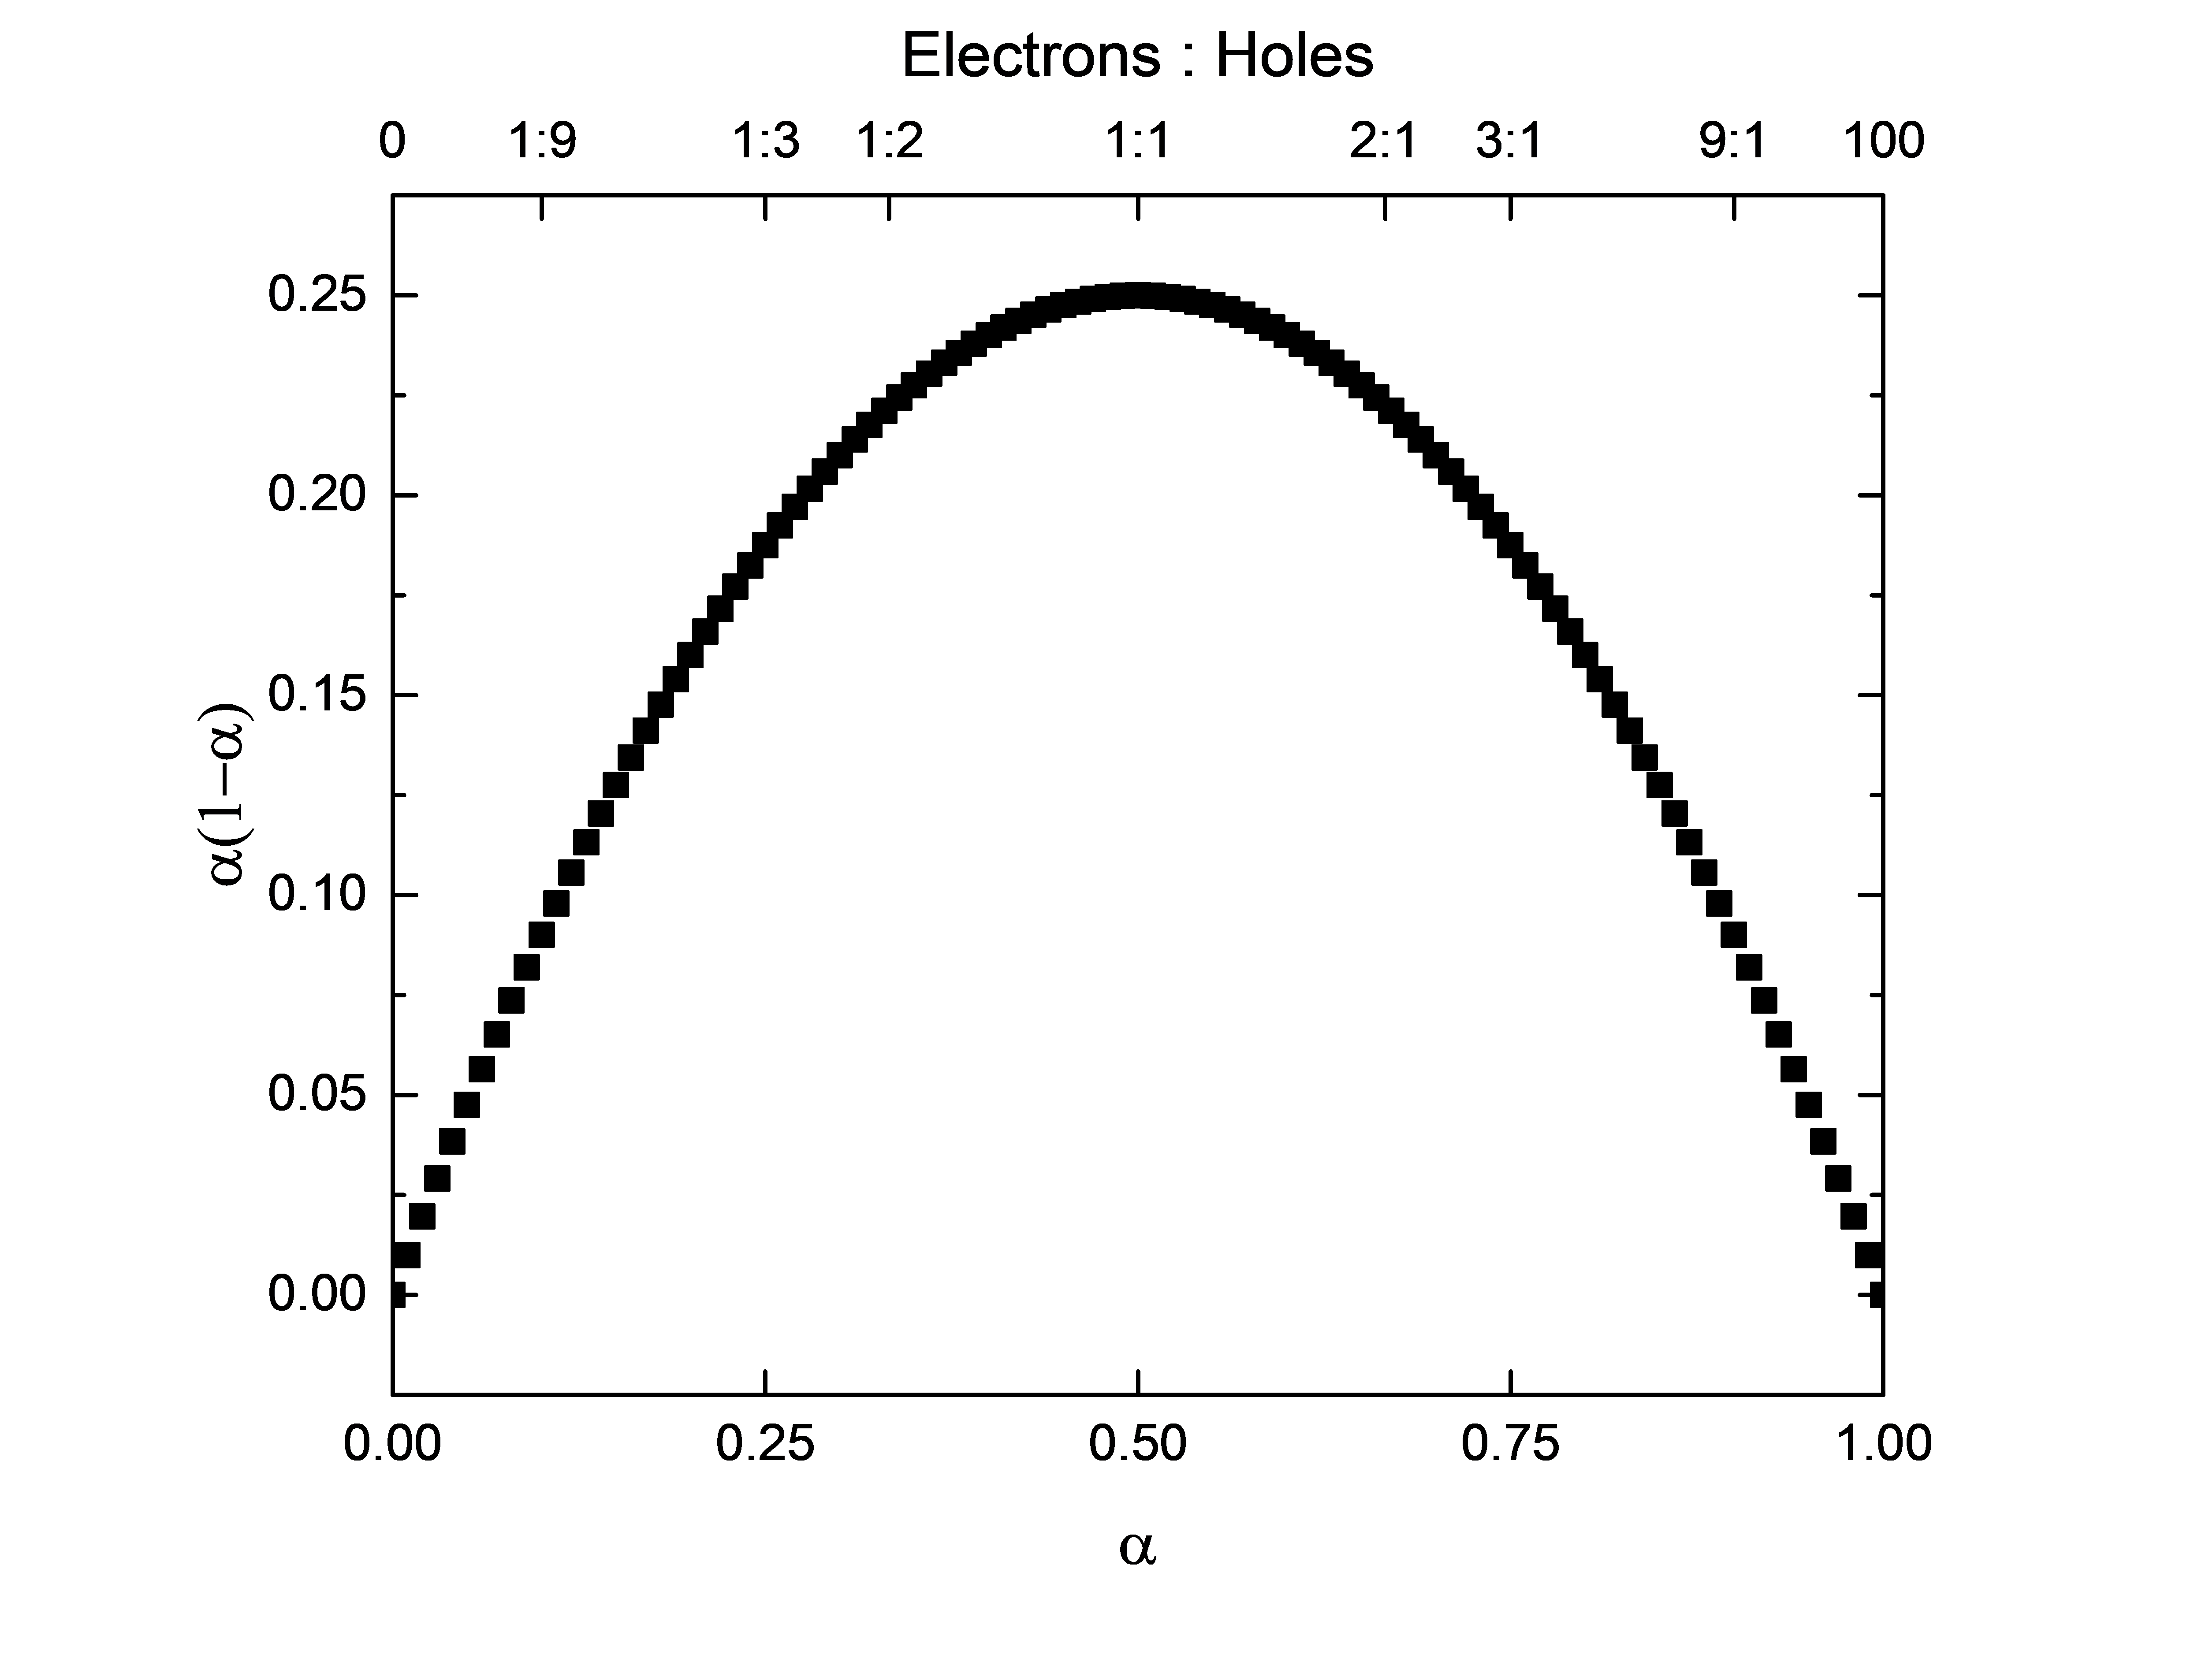
\includegraphics[scale=.1]{unified/EHratio}
\caption{The quantity $\alpha(1-\alpha)$ is plotted as a function of the polaron composition, $\alpha$ and the electron to hole ratio.}
\label{fig:EHratio}
\end{wrapfigure}

\ifcsdef{mainfile}{}{\bibliography{../library}}
\end{document}

